\subsection{Свободная, 	вынужденная, переходная и установившаяся составляющие движения дискретной системы}
Аналитическое решение уравнения:
\begin{equation}
    y(k) = y_\text{св}(k) + y_\text{в}(k)
\end{equation}
Выражение содержит вынужденную составляющую  $y_\text{в}(k)$, соответствующую реакции системы на входное воздействие $u(k)$, и свободную составляющую $ y_\text{cв}(k)$, соответствующую решениям однородного разностного уравнения (автономной дискретной системы): $a0 y(k+n) + a1 y(k+n-1) +\dots+ an y(k) = 0$ при начальных условиях $y(0), у(-1), \dots, у(-n+1)$.

Поведение системы и свободная составляющая переходного процесса зависят от полюсов системы $z_i$, которые в общем случае представлены комплексно-сопряженными парами:
\begin{gather}
    z_{i,i+1} = \alpha_i \pm j \beta_i = M_i e^{\pm \psi},\\
    M_i = |z_{i,i+1}| = \sqrt{\alpha_i^2 + \beta_i^2}, \\
    \psi_i = \arg z_{i, i+1} = \arctan{(\cfrac{\beta_i}{\alpha_i})}
\end{gather}
\begin{equation}
    y_{\text{св}}(k) = C_1 z_1^k + C_2 z_2^k + \dots + C_n z_n^k    
\end{equation}
где $C_i$~--- неопределенные коэффициенты, зависящие от начальных условий.
\begin{enumerate}
    \item Для вещественных корней $\alpha > 0, \beta = 0, \psi = 0$ соответствует апериодическаая составляющая переходного процесса (мода)
    \begin{equation}
        y_i(k) = C_i M_i^k
    \end{equation}
    
    \item Для вещественных корней $\alpha < 0, \beta = 0, \psi = \pi$ соответствует колебательная  мода
    \begin{equation}
        y_i(k) = C_i M_i^k \cos{(k \pi)}
    \end{equation}
    
    \item Паре комплексно-сопряженных соответстует колебательная составляющая
    \begin{equation}
        y_i(k) = A_i M_i^k \cos{(k \psi_i - \phi_i)}
    \end{equation}
    где $A_i, \phi_i$~--- параметры зависящие от начальных условий.
\end{enumerate}

Если при некторых начальных условиях имеет место тождество:
\begin{equation}
    \y_{\text{св}} (k) = y^* = const, k > 0,
\end{equation}
то значение $y^*$ называют положением равновесия автономной системы.

Вынужденная составляющая переходного процесса определяется входным воздействием $u(k)$. Наиболее распространенными входными сигналами дискретных систем являются единичная импульсная последовательность и дельта-функция Кронекера.

\textbf{Переходные процессы.}
\begin{figure}
    \centering
    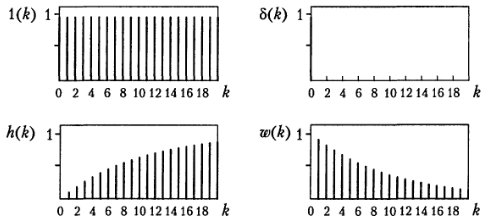
\includegraphics[width=0.5\linewidth]{images/input/kt.png}
    \caption{Caption}
    \label{fig:my_label}
\end{figure}

При нулевых начальных условиях системы:
\begin{equation}
    h(0) = \dots = h(-n+1) = 0, w(0) =  \dots = w(-n+1) = 0
\end{equation}
Единичная импульсная последовательность:
\begin{equation}
    \mathbf{1}(k) =
    \begin{cases}
    0, k < 0, \\
    1, k \ge 0.
    \end{cases},
    \quad
    h(k) = y(k)|_{y_o(k) = 0, u(k) = \mathbf{1}(k)} = y_{\text{в}}
\end{equation}

Дельта функция:
\begin{equation}
    \mathbf{\delta}(k) =
    \begin{cases}
    0, k \ne 0, \\
    1, k = 0.
    \end{cases},
    \quad
    w(k) = y(k)|_{y_o(k) = 0, u(k) = \mathbf{\delta}(k)} = y_{\text{в}}
\end{equation}

\textbf{Установившаяся составляющая.}
\begin{equation}
    y_{\text{у}} = \cfrac{b_1 + \dots + b_n}{1+a_1 + \dots + a_n} u = K u = W(1) u
\end{equation}
где $K$~--- \textit{статический коэффициент}.

Условие существования статической характеристики:
\begin{equation}
    1+a_1 + \dots + a_n \ne 0
\end{equation}
и система удовлетворяющая этому условию называетя статической.




